\subsection{Characterisation of CD14$^+$ monocyte heterogeneity in PsA using scRNA-seq}
According to the analysis of chromatin accessibility and immune-related gene expression in this pilot cohort, CD14$^+$ monocytes showed the largest number of significant DARs and the most reliable modulation of expression, highlighting changes in expression between peripheral blood and synovial fluid for pro-inflammatory chemokines and cytokines. Monocytes are very plastic cells which initiate differentiation into macrophages at the site of inflammation. Therefore, exploring differences at the single-cell level may identify subpopulations with particular phenotypes of interest and may also highlight differences in the immune response driven by this cell type in circulation and at the inflamed synovium.


\subsubsection{Combined scRNA-seq analysis of synovial fluid and peripheral blood CD14$^+$ monocytes reveals two main subpopulations}
%Explain how I did the analysis
scRNA-seq was performed in paired PBMCs and SFMCs isolated from three PsA patients (Table \ref{tab:PSA_datasets_per_sample}). scRNA-seq data from each of the PBMCs and SFMCs samples were donwsampled to 3,500 cells and filtered to remove cells with abundant mitochondrial reads and excessive number of unique molecular identifiers (UMI), and genes expressed in low number of cells (as explained in Chapter \ref{ch:Mat}). CD14$^+$ monocytes were distinguished from other cell populations by expression of \textit{CD14} and \textit{LYZ}, two of the most accurate expression markers defining this cell population (Figure \ref{figure:PsA_scRNAseq_SF_an_PB_monocytes_identification_from_bulk}A and B). Across all 6 samples (3 SFMCs and 3 PBMCs), 2,459 cells were CD14$^+$ monocytes cells, representing approximately 17\% of the bulk SFMCs and PBMCs cells included in the analysis and in line with the proportion of CD14$^+$ monocytes previously reported using cell surface markers by mass cytometry  (Figure \ref{figure:PsA_cell_composition}). The CD14$^+$ monocytes identified in each of the 3paired PBMCs-SFMCs PsA samples were combined using canonical correlation analysis to correct for intrinsic batch effect, unavoidable due to patient samples recruitment on different days and generation of SFMCs and PBMCs 10X libraries separately. CCA alignment of the six CD14$^+$ monocytes populations was followed by conservative unsupervised clustering (using resolution 0.1) and t-SNE visualisation. 



\bigskip
\begin{figure}[H]
\centering
\begin{subfigure}[b]{0.60\textwidth}
\centering 
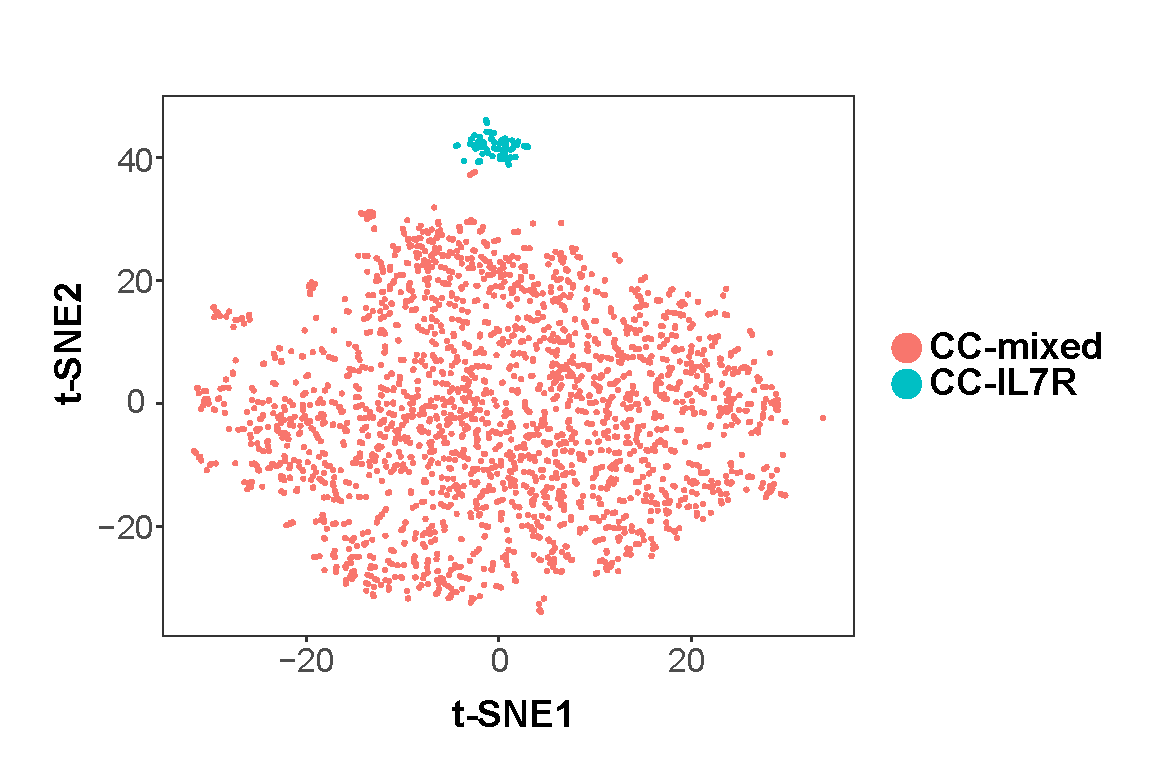
\includegraphics[width=\textwidth]{./Results3/pdfs/PSA_scRNAseq_tSNE_CC_mixed_and_IL7R}
\caption{}
\end{subfigure}
~
\begin{subfigure}[b]{0.75\textwidth} 
%the [b] prevents offset in subcaptions
\centering
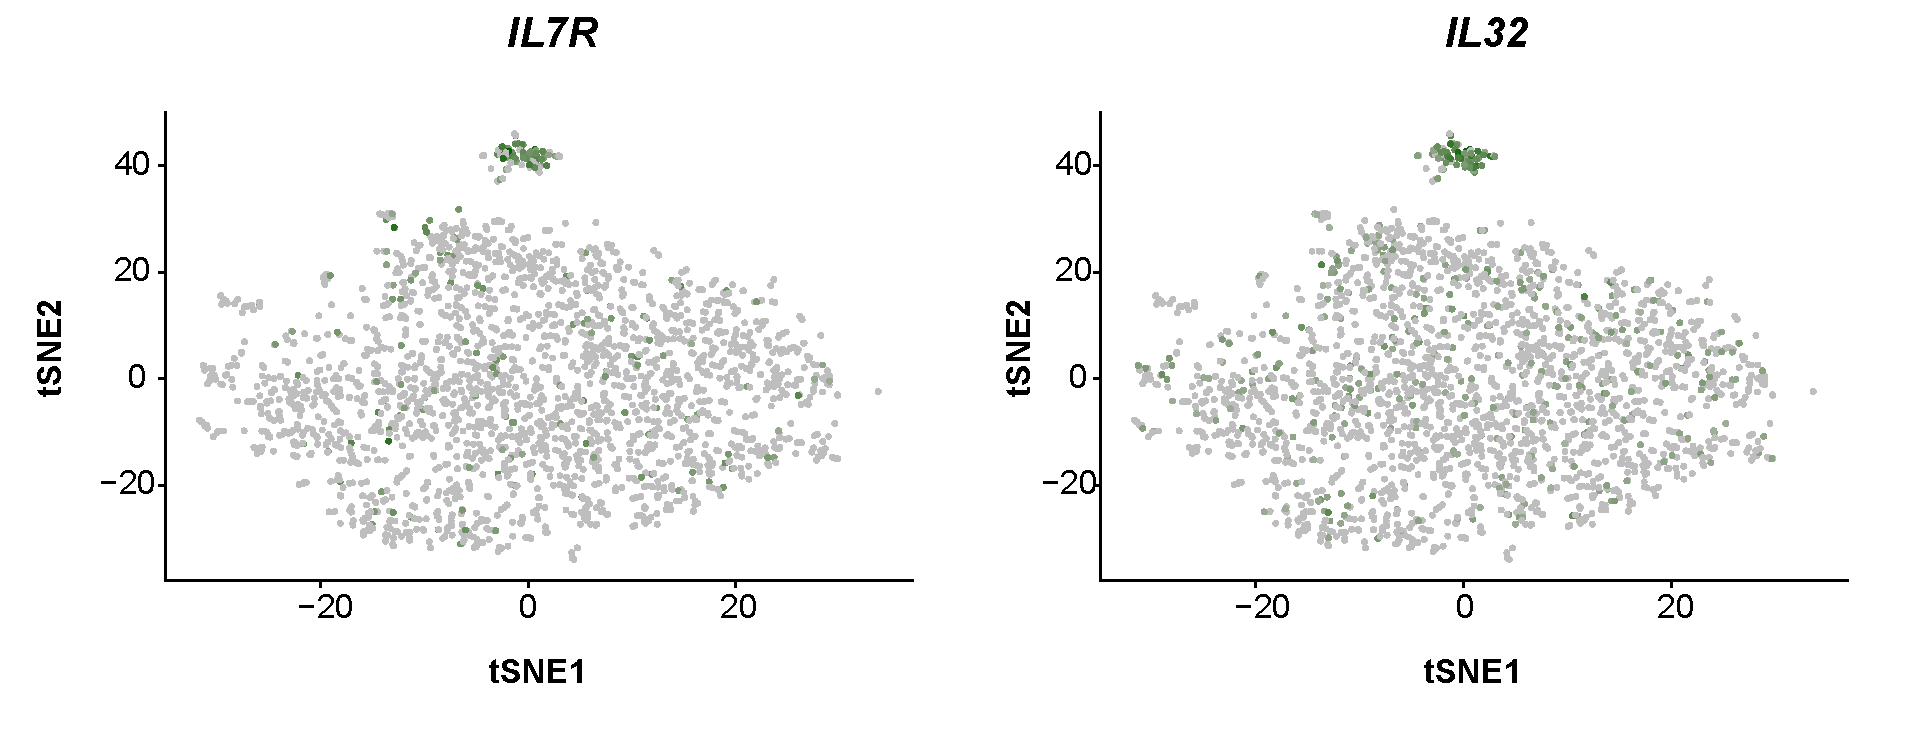
\includegraphics[width=\textwidth]{./Results3/pdfs/PSA_scRNAseq_CC_mixed_and_IL7R_overlay_markers}
\caption{}
\end{subfigure}
\caption[Identification of two main CD14$^+$ monocytes subpopulations in the synovial fluid and peripheral blood combined analysis]{\textbf{Identification of two main CD14$^+$ monocytes subpopulations in the synovial fluid and peripheral blood combined analysis.} (A) Visualisation using t-SNE dimensional reduction of the two cluster (CC-mixed and CC-IL7R) identified in the combined synovial fluid and peripheral blood CD14$^+$ monocyte cells using a very conservative resolution (res=0.1) for the unsupervised clustering analysis. Each of the dots represents a cell, colour-coded by the cluster membership (pink=CC-mixed and turquoise=CC-IL7R). (B) Overlap of \textit{IL7R} and \textit{IL32} expression intensities (green) on the t-SNE representation of the synovial fluid and peripheral blood CD14$^+$ monocytes. \textit{IL32} and \textit{IL7R} gene expression appeared as markers for the CD14$^+$ monocytes from the CC-IL7R cluster.}
\label{figure:PsA_scRNAseq_SF_an_PB_monocytes_identification_from_bulk}
\end{figure}

%Say that using a conservative approach to find cluster two main groups were identified: No IL7R vs IL7R
%Probably more heterogeneity could be found within the big cluster but given number of replicates and intensive analysis required to make sure clusters are estable we decided to only trust these two main groups
Using this conservative approach for cluster definition, two robust clusters were identified (Figure \ref{figure:PsA_scRNAseq_SF_an_PB_monocytes_identification_from_bulk} a). The smallest cluster, named CC-IL7R, was characterised by the expression of \textit{IL7R}, \textit{IL32} and \textit{CCL5}, amongst others, and was formed by a total of 72 cells (43 from synovial fluid versus 29 from peripheral blood) (Figure \ref{figure:PSA_scRNAseq_CC_mixed_and_IL7R_overlay_markers} b and \ref{figure:PSA_scRNAseq_CC_mixed_and_IL7R_markers_heatmap}). The proportion of IL7R$^+$CD14$^+$ monocytes when compared to the total CD14$^+$ monocyte population was very similar in synovial fluid and peripheral blood (3 and 2.7\%, respectively) in this data. This did not reflect the differences in the number of CD14$^+$ IL7R$^+$ monocytes identified using FACS (in revision Al-Mossawi \textit{et al.}, 2018). The largest cluster, named as CC-mixed, consisted of 2,387 (1,356 synovial fluid and 1,031 peripheral blood). CC-mixed was an heterogeneous cluster, without consistent expression pattern for those genes identified as cluster markers (Figure \ref{figure:PSA_scRNAseq_CC_mixed_and_IL7R_markers_heatmap}). When using a less conservative approach for cluster definition by increasing the resolution (resolution 0.4, 0.6 and 0.8), additional clusters were identified. Similarly to the observation in the most conservative approach, no consistency was found in the expression of the top genes defined as markers by cells of the same cluster (data not shown). Downstream analysis, including DGE between the two tissues, was performed in the CC-mixed and CC-IL7R clusters identified by the most conservative approach (resolution 0.1).
%Due to the moderate cohort size, limitation in accounting for batch effect for cluster identification and the complexity in the definition and identification of stable clusters this analysis could only yield limited information about monocytes subpopulations. Increasing cohort size and a implementation of more exhaustive analysis and alternative methods could lead to identification of additional subpopulations within the combined synovial fluid and peripheral blood CD14$^+$ monocytes in the CC-mixed cluster (see \ref{Discussion_scRNAseq}). For the scope of this project, downstream analysis, including DGE between the two tissues, was performed in the CC-mixed and CC-IL7R clusters identified by the most conservative approach (resolution 0.1).




\subsubsection{Differential gene expression between synovial fluid and peripheral blood CD14$^+$ monocytes in CC-mixed and CC-IL7R}
%DGE was performed between tissues within each cluster
DGE analysis was performed in order to explore differences between synovial fluid and peripheral blood within each of these two main CD14$^+$ monocyte subpopulations. For the CC-mixed cluster, a total of 251 genes were differentially expressed at an FDR$<$0.01 and fold change$>$1.5 between synovial fluid and peripheral blood, of which 149 and 102 showed up- and down-regulation, respectively (Figure \ref{figure:PsA_scRNAseq_vulcano_plots_mixed_and_IL7R_clusters} a). Differential analysis within the CC-IL7R cluster revealed a total of 37 modulated genes, with the majority (35 out of 37) up-regulated in synovial fluid compared to peripheral blood (Figure \ref{figure:PsA_scRNAseq_vulcano_plots_mixed_and_IL7R_clusters} a). Due to the low number of cells in the CC-IL7R cluster and the limited sample size (n=3), the analysis only identified as significantly differentially expressed (FDR$<$0.01) genes presenting fold change$>$1.5. Out of the 37 DEGs in the CC-IL7R cluster between the two tissues, 30 were also shared by the CC-mixed cluster. The seven distinctly modulated genes in the CC-IL7R cluster included \textit{CD44} (receptor of the protein product of \textit{SPP1}), \textit{MT-CO2} or S-ribosomal protein (RPS) genes (\textit{RPS29} and \textit{RPS27}). 


\bigskip
\begin{figure}[H]
\centering
\begin{subfigure}[b]{0.55\textwidth}
\centering 
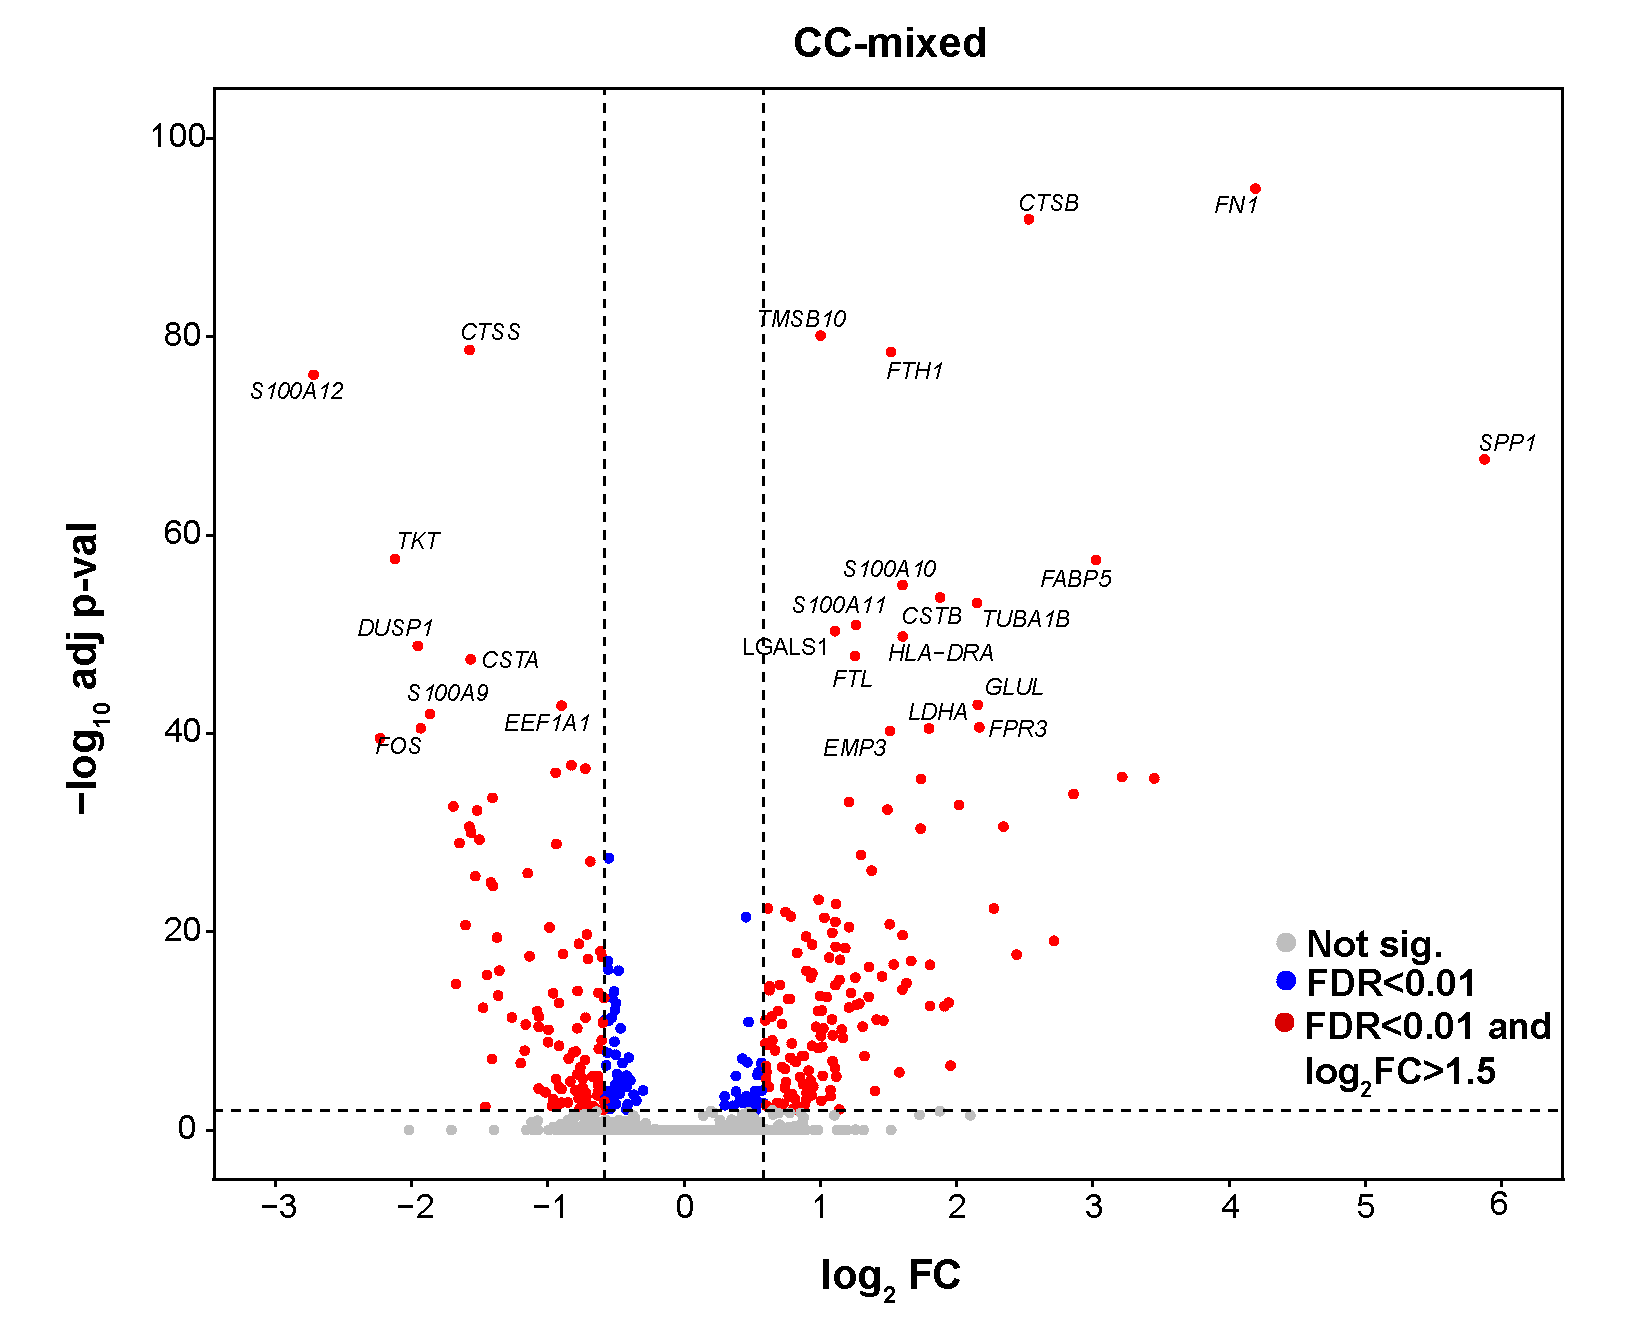
\includegraphics[width=\textwidth]{./Results3/pdfs/PSA_10X_all_combined_aligned_monocytes_DGE_SF_vs_PB_cluster_0_vulcano_plot}
\caption{}
\end{subfigure}
~
\begin{subfigure}[b]{0.55\textwidth} 
%the [b] prevents offset in subcaptions
\centering
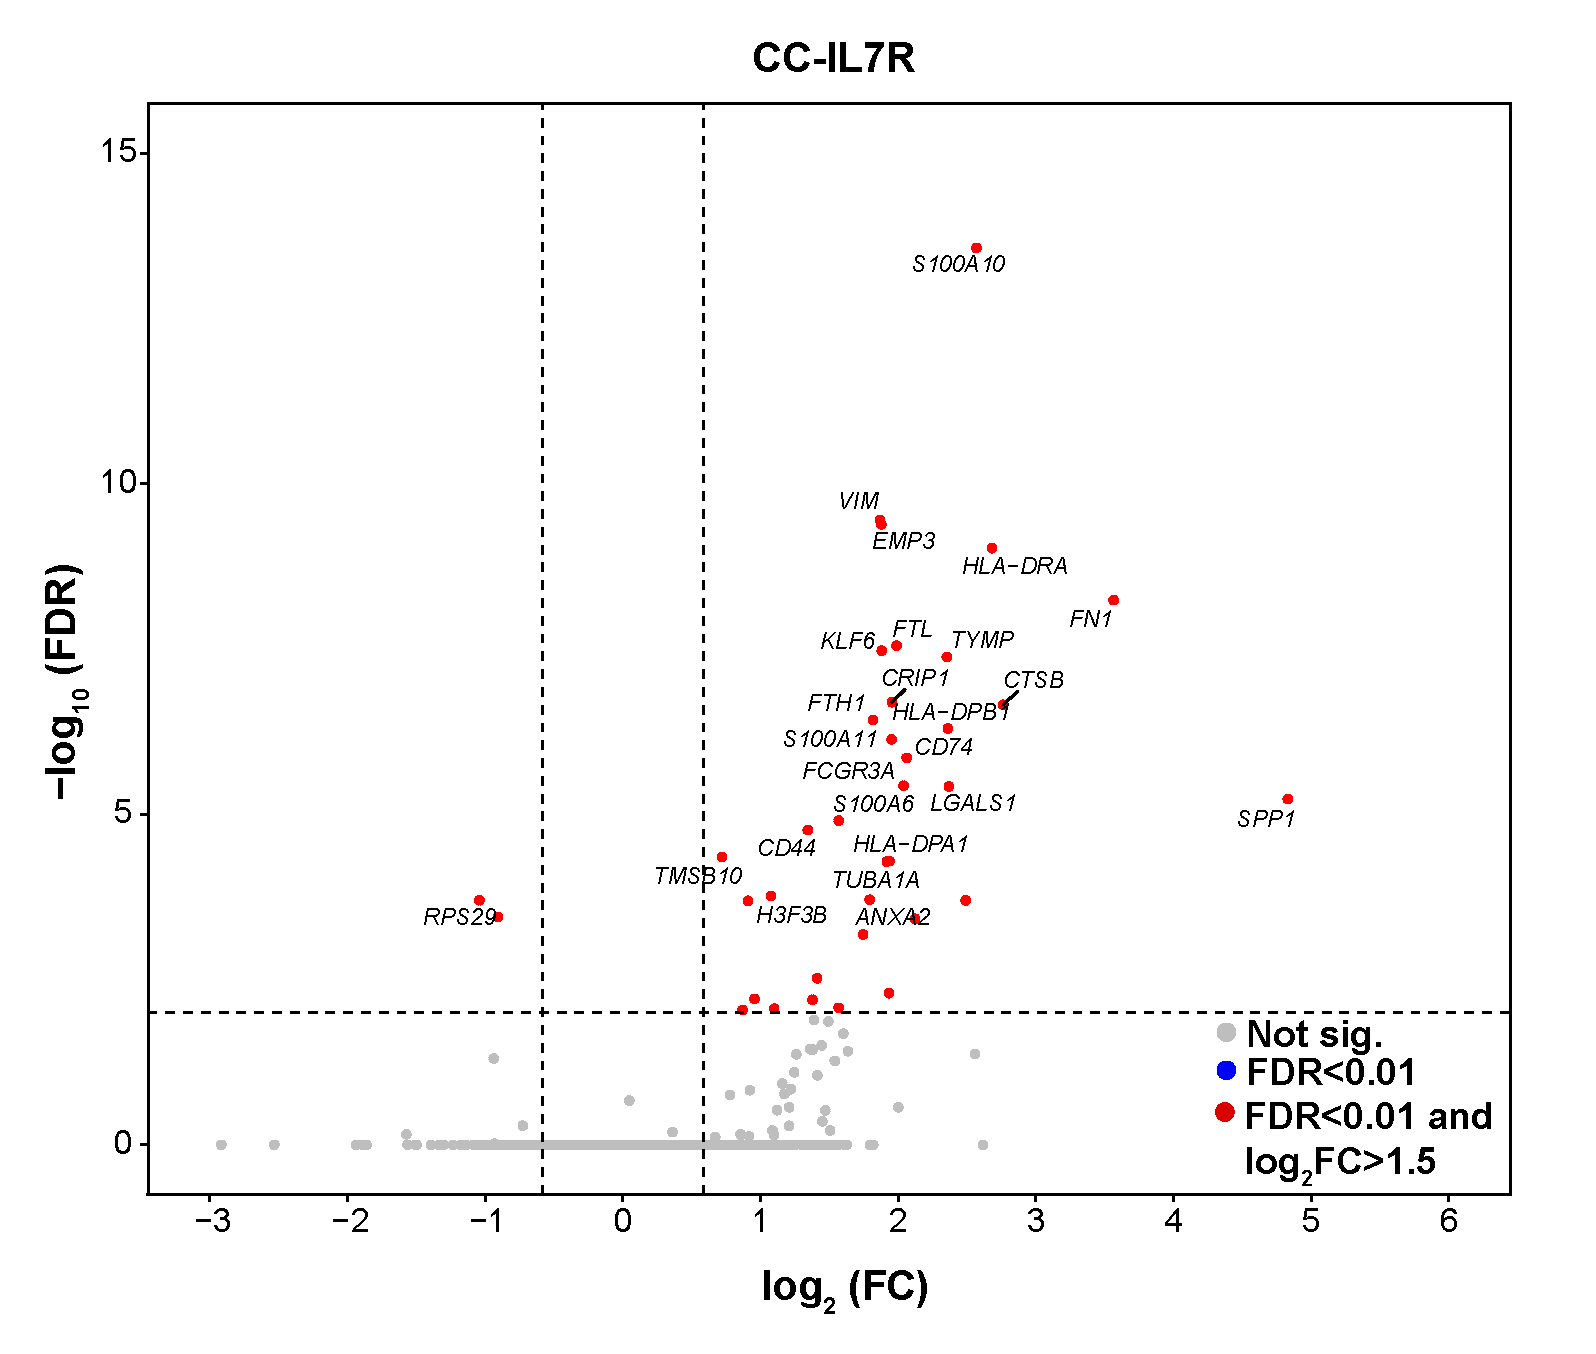
\includegraphics[width=\textwidth]{./Results3/pdfs/PSA_10X_all_combined_aligned_monocytes_DGE_SF_vs_PB_IL7R_vulcano_plot}
\caption{}
\end{subfigure}
\caption[Sc-RNA-seq differential gene expression results between synovial fluid and peripheral blood in the CC-mixed and CC-IL7R CD14$^+$ monocytes subpopulations.]{\textbf{Sc-RNA-seq differential gene expression results between synovial fluid and peripheral blood in the CC-mixed and CC-IL7R CD14$^+$ monocytes subpopulations.} Vulcano plots showing differences in gene expression between synovial fluid and peripheral blood in the (A) CC-mixed and (B) CC-IL7R CD14$^+$ monocyte clusters. In A and B, the significance (log$_{10}$FDR) of the differential expression (y-axis) is plotted against the log${_2}$fold change. A positive fold change indicates higher expression in CD14$^+$ monocytes from synovial fluid compared to peripheral blood. Genes showing FDR$<$0.01 are coloured in blue and genes presenting and FDR$<$0.01 and fold change$>$1.5 are coloured in red. The most significant genes are labelled.}
\label{figure:PsA_scRNAseq_vulcano_plots_mixed_and_IL7R_clusters}
\end{figure}



Comparison with the qPCR expression analysis revealed a modest overlap between the two assays, particularly for the DEGs in the CC-IL7R. Amongst the 72 DEGs (p-value$<$0.05) detected by qPCR between synovial fluid and peripheral blood in CD14$^+$ monocytes, only 12 and 4 genes were also differentially expressed (FDR$<$0.01 and no fold change threshold) in the CC-mixed and CC-IL7R clusters, respectively (Figure \ref{figure:PsA_scRNAseq_qPCR_ATAC_correlation}A). Genes with reproducible differential expression between synovial fluid and peripheral blood by the two approaches included genes with the largest fold changes in both assays, such as \textit{SSP1}, \textit{FN1}, \textit{OLR1} and \textit{S100A12}, being the direction of change also consistent for all of them. %add something about cell type specificity
%Regarding the low number of qPCR DEGs between synovial fluid and peripheral blood in total CD14$^+$ monocytes reproduced by the scRNA-seq in any of the two main clusters identified could be explained by the differences in the cell sorting (FACS versus \textit{in silico} expression markers), the low number of replicates for each assay as well as different sensitivity of the two technologies. 
%The limited overlap between qPCR and scRNA-seq DEGs could also partly explain the absence of overlap between enriched pathways across the two gene expression analysis. 
   
\bigskip
\begin{figure}[H]
\centering
\begin{subfigure}[b]{0.50\textwidth}
\centering 
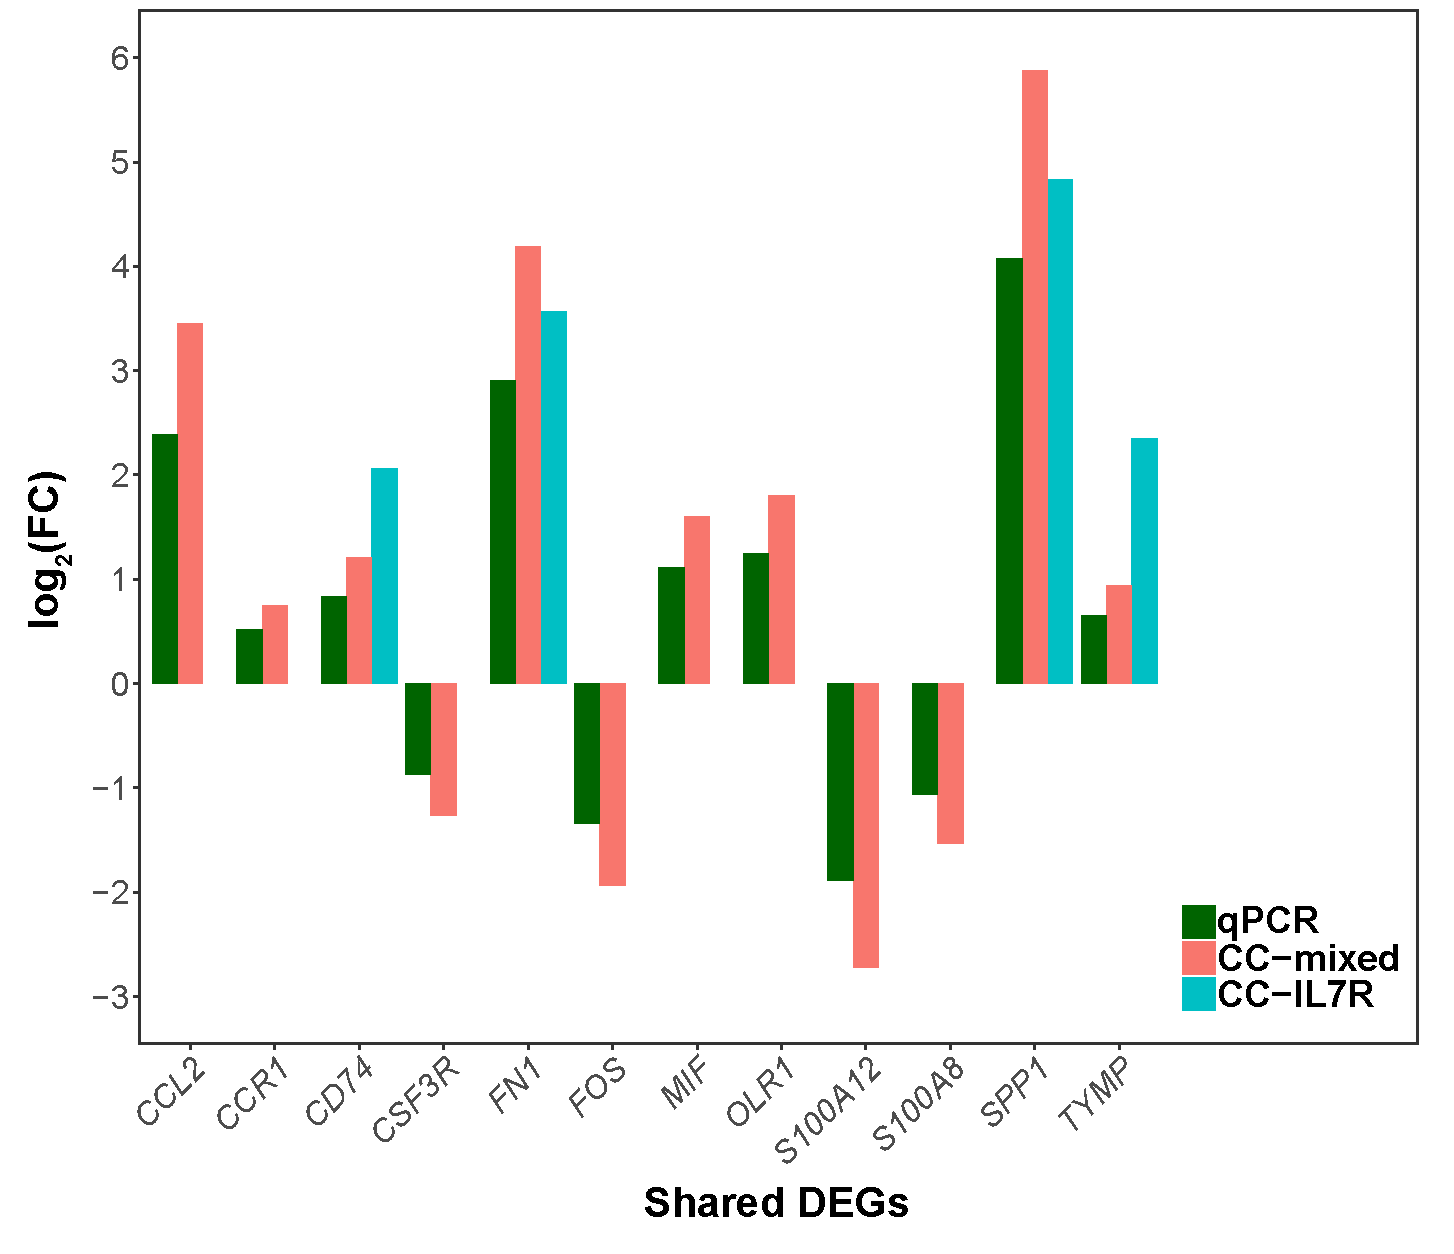
\includegraphics[width=\textwidth]{./Results3/pdfs/PSA_scRNAseq_PCR_array_overlapping_genes_log2FC}
\caption{}
\end{subfigure}
~
\begin{subfigure}[b]{0.70\textwidth} 
%the [b] prevents offset in subcaptions
\centering
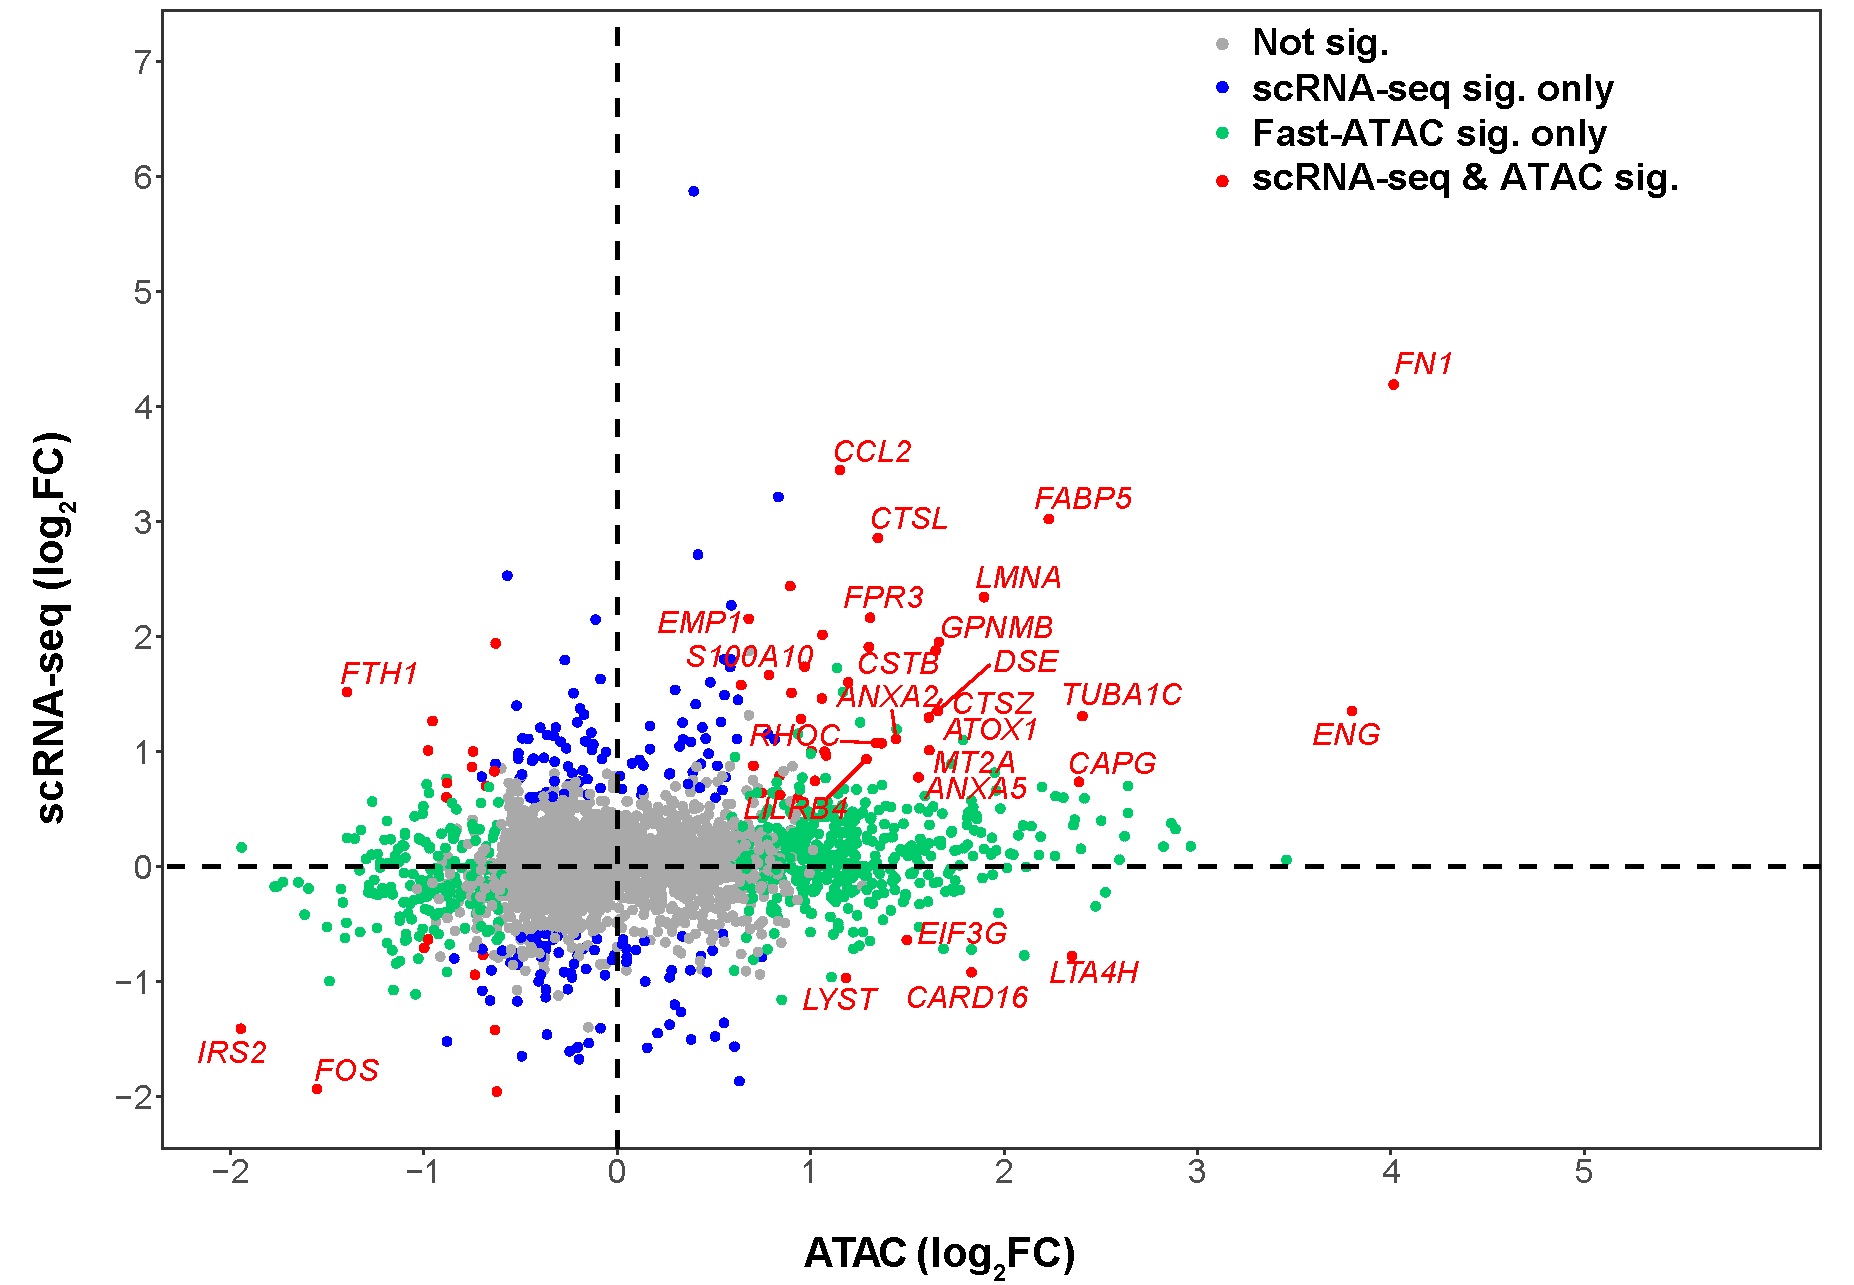
\includegraphics[width=\textwidth]{./Results3/pdfs/PSA_ATAC_scRNA_CD14_correlation_plot}
\caption{}
\end{subfigure}
\caption[Correlation between scRNA-seq, qPCR and chromatin accessibility in PsA CD14$^+$ monocytes.]{\textbf{Correlation between scRNA-seq, qPCR and chromatin accessibility in PsA CD14$^+$ monocytes.} (A) Overlap between the scRNA-seq DEGs (significant based only on FDR$<$0.01) from the CC-mixed and CC-IL7R CD14$^+$ monocyte cluster in synovial fluid versus peripheral blood and the corresponding DEGs (p-value<0.05) detected by qPCR in the bulk CD14$^+$ monocytes population. For each of the shared DEGs, the log$_2$fold changes from the qPCR and the 10X scRNA-seq analysis are represented. (B)Correlation plot comparing synovial fluid and peripheral blood differences in scRNA-seq expression of the CC-mixed CD14$^+$ monocytes and ATAC chromatin accessibility in total CD14$^+$ monocytes. The log$_2$fold changes for scRNA-seq differential expression of all transcripts in the CC-mixed CD14$^+$ monocytes are plotted against the log$_2$fold change for total CD14$^+$ monocytes ATAC differential chromatin accessibility analysis in regions proximal ($\leq$5Kb) to the same genes. Blue colouring indicates significant differential expression in scRNA-seq only; green represents ATAC significant DAR only; red indicates significant differential expression and chromatin accessibility; grey indicates no significant differential expression or chromatin accessibility in CD14$^+$ monocytes. Significance is based on FDR and fold change thresholds (FDR$<$0.01 and fold change$>$1.5) in both assays.}
\label{figure:PsA_scRNAseq_qPCR_ATAC_correlation}
\end{figure}


%Interestingly, latest studies have involved RPS proteins in immune signalling and modulation of the NF-$\kapa$B response \parencite{Zhou2015}


% Pathway analysis
Pathway enrichment analysis was performed for the significantly DEGs between synovial fluid and peripheral blood in the CC-mixed and CC-IL7R subpopulations. The DEGs in the CC-mixed cluster were significantly enriched (FDR$<$0.01) a number of pathways (Table \ref{tab:PSA_scRNAseq_CD14_DEGs_pathway_analysis} and \ref{tab:PSA_scRNAseq_CC_mixed_and_IL7R_additional_pathways}), some of them of particular pathological relevance (Table \ref{tab:PSA_scRNAseq_CD14_DEGs_pathway_analysis}). 

\begin{table}[htbp]
%\setlength{\tabcolsep}{20pt} only to stretch the columns if you want
%\renewcommand{\arraystretch}{1.5}
\centering
\begin{tabular}{@{} c c c}
\toprule
\textbf{Cluster} & \textbf{Pathways} \\
\midrule
\midrule
         & Ag processing and presentation via MHC-II \\
				 & Extracellular matrix and extracellular \\
				 & matrix-associated proteins \\
CC-mixed & Phagosome and lysosome formation \\
				 & IFN signalling \\
				 & Cytokine signalling $^\ast$ \\
				 & Apoptosis \\
				 & Innate immunity \\
\midrule				
         & Adaptive immunity \\
         & Ag processing and presentation \\
CC-IL7R	 & Phagosome \\
         & Extracellular matrix and extracellular \\
				 & matrix-associated proteins \\
\bottomrule
\end{tabular}
\medskip %gap
\caption[Most relevant enriched pathways for the DEGs between synovial fluid and peripheral blood CD14$^+$ monocytes in CC-mixed and CC-IL7R.]{\textbf{Most relevant enriched pathways for the DEGs between synovial fluid and peripheral blood CD14$^+$ monocytes in CC-mixed and CC-IL7R.} Significantly DEGs based on the FDR and fold change threshold were used for the analysis. Most relevant enriched pathways based on FDR$<$0.01. $^\ast$ Enrichment for FDR$<$0.05. Additional pathways included in Table \ref{tab:PSA_scRNAseq_CC_mixed_and_IL7R_additional_pathways}.}
\label{tab:PSA_scRNAseq_CD14_DEGs_pathway_analysis}
\end{table}


One of those pathways was for the Ag processing and presentation pathway, contributed by up-regulated expression in synovial fluid CD14$^+$ monocytes of \textit{CD74} and genes from the \textit{HLA-D} family such as \textit{HLA-DQA1} and \textit{HLA-DRB1} (Table \ref{tab:PSA_scRNAseq_CD14_DEGs_pathway_analysis}). Enrichment for IFN signalling was driven differential expression of genes such as \textit{IFI6}, \textit{IFITM3}, \textit{ISG15} and the TF \textit{STAT1}, all of them up-regulated in synovial fluid when compared to peripheral blood CD14$^+$ monocytes. Another relevant enriched pathway was the extracellular matrix and extracellular matrix-associated proteins, which involve genes of the S100 family (including \textit{S100A8}, \textit{S100A9}, \textit{S100A10}, \textit{S100A11} and S100A12, that interact with the receptor for advance glycosylation end products (RAGE) and induce production of matrix-degrading enzymes. The phagosome and lysosome formation pathway also appeared to be more active in synovial fluid CD14$^+$ monocytes, with up-regulation of genes such as \textit{CTSL}, which is involved in protein degradation in lysosomes and phagocytosis of apoptotic cells. Lastly, enrichment for cytokine signalling was not driven by differential expression of cytokines but was contributed by up-regulation of pro-inflammatory TFs such as \textit{STAT1}, amongst other genes. The most functionally relevant significantly enriched pathways identified for DEGs in the CC-IL7R subpopulation were common to the ones found in the CC-mixed cluster (Table \ref{tab:PSA_scRNAseq_CD14_DEGs_pathway_analysis}).



\subsubsection{Moderate genome-wide correlation correlation between chromatin accessibility and scRNA-seq expression in the CC-mixed cluster}
In order to determine the overall correlation between scRNA-seq expression and chromatin accessibility, comparison between the log$_2$fold changes for all the expressed genes in the CC-mixed CD14$^+$ monocytes cluster and all the accessible chromatin regions in bulk CD14$^+$ monocytes between synovial fluid and peripheral blood was conducted . Changes in expression and chromatin accessibility only showed a moderate correlation in this data (R=0.214, p-value=2x10$^{-16}$) (Figure \ref{figure:PsA_scRNAseq_qPCR_ATAC_correlation}B). In the CC-mixed cluster, 64 genes out of the 251 DEGs (FDR$<$0.01 and fold change$>$1.5) were proximal ($\leq5$Kb) to one or more ATAC DARs (Table \ref{tab:PSA_10X_CD14_clusters_and_ATAC_overlap}). This overlap was significant and highlighted the enrichment (Fisher exact test p-value=1.5x10$^-3$) of DEGs in the CC-mixed cluster for proximal DARs identified by ATAC in bulk CD14$^+$ monocytes. The majority of the overlaps corresponded to matched increase or decrease (40 and 12 genes, respectively) of gene expression and chromatin accessibility in synovial fluid vs peripheral blood. However, 14 DEGs in the CC-mixed cluster showed opposite direction of change between expression and chromatin accessibility (Table \ref{tab:PSA_10X_CD14_clusters_and_ATAC_overlap}). 


  
\begin{table}[htbp]
%\setlength{\tabcolsep}{20pt} only to stretch the columns if you want
%\renewcommand{\arraystretch}{1.5}
\centering
\begin{tabular}{@{} c c c c}
\toprule
\textbf{Cluster} & \textbf{Up-regulated genes}       &  \textbf{Up-regulated genes }     & \textbf{Opposite direction} \\
                 & \textbf{with proximal}            &  \textbf{with proximal}           & \textbf{in expression } \\
								 &	\textbf{synovial fluid}				   &  \textbf{peripheral blood}        & \textbf{and DAR}         \\
								 &	\textbf{open DAR}				         &  \textbf{open DAR}                &                           \\
\midrule
\midrule
 CC-mixed         & 40                                       &  10                                & 14 \\
 CC-IL7R          & 9                                        &  0                                 & 4 \\
\bottomrule
\end{tabular}
\medskip %gap
\caption[scRNA-seq DEGs in synovial fluid versus peripheral blood CD14$^+$ monocytes proximal to a DAR in Fast-ATAC.]{\textbf{scRNA-seq DEGs in synovial fluid versus peripheral blood CD14$^+$ monocytes proximal to an ATAC DAR.}. For each of the two CD14$^+$ monocytes cluster identified by scRNA-seq analysis, an overlap is defined when a gene is differentially expressed (FDR$<$0.01 and fold change$>$1.5) between synovial fluid and peripheral blood and a proximal significant DAR ($\leq$5Kb) showing same or opposite direction of change is also found.}
\label{tab:PSA_10X_CD14_clusters_and_ATAC_overlap}
\end{table}

Amongst the DEGs in the CC-mixed cluster overlapping a proximal DAR were \textit{CCL2} and \textit{FN1} (Figure \ref{figure:PsA_scRNAseq_qPCR_ATAC_correlation}B). Both genes were up-regulated in synovial fluid compared to peripheral blood in the CC-mixed cluster, proximal to a synovial fluid open DAR, and found up-regulated in the same direction by the qPCR expression analysis in synovial fluid bulk CD14$^+$ monocytes compared to peripheral blood (Figure \ref{figure:PsA_scRNAseq_qPCR_ATAC_correlation}A). 

Similarly to the CC-mixed results, the DEGs in the CC-IL7R cluster between synovial fluid and peripheral blood were also enriched for those genes with at least one DARs nearby (Fisher exact test p-value=1.85x10$^-9$). Amongst the 22 DEGs overlapping a proximal DAR, 13 of them had correlated dysregulation of expression and chromatin accessibility only 4 presented opposite directionality in the variation of the two features (Table \ref{tab:PSA_10X_CD14_clusters_and_ATAC_overlap}). 


\ToDo{Overall, this results have shown only moderate correlation between gene expression and proximal chromatin accessibility. For some genes this correlation may highlight the relationship between the changes in chromatin accessibility and gene expression observed in synovial fluid and peripheral blood in CD14$^+$ monocytes. However, functional investigation will be required to establish this relationship.}





%The biological relevance of the IL7R does not show distinct differences in gene expression between tissues and its relevance may be related to the distinctive biological function of this subset in both tissues. Seems more abundant in synovial fluid and that would make sense with the differences in the PCR array in bulk expression.
